% Tipo de documento
\documentclass[12pt,a4paper]{article}

% Pacotes
%\usepackage{showlabels}
\usepackage{latexsym}
\usepackage{amsfonts}
\usepackage{amsmath}
\usepackage{amscd}
\usepackage[brazil]{babel}
\usepackage[utf8]{inputenc}
\usepackage[pdftex]{graphicx} 

% Paginação
%\textwidth 15.0cm                    % Largura
%\textheight 22.0cm                   % Altura
%\addtolength{\oddsidemargin}{0.0cm}  % Margem esquerda (impar)
%\addtolength{\evensidemargin}{0.0cm} % Margem esquerda (par)
%\addtolength{\topmargin}{0.0cm}      % Margem superior

% Estilo dos parágrafos
\sloppy                              % Mais flexível
\setlength{\jot}{08pt}               % Distância entre linhas do eqnarray
\setlength{\parskip}{1ex}            % Distância entre parágrafos
\renewcommand{\baselinestretch}{1.0} % Distância entre linhas

% Comandos customizados
\newcommand{\vet}{\mathbf}                                   % vetor
\newcommand{\ie}{\emph{i.e.}}                                % isto é
\newcommand{\prodint}[2]{\left\langle #1 , #2 \right\rangle} % produto interno
\newcommand{\Fullbox}{{\rule{2.0mm}{2.0mm}}}                 % caixa cheia
\newcommand{\EOS}{\hfill\Box\vspace{-0.2cm}}                 % fim de enunciado
\newcommand{\EOP}{\hfill\Fullbox\vspace{0.2cm}}              % fim de prova
\newcommand{\eps}{\varepsilon}                               % epsilon
\newcommand{\defi}{\: := \: }                                % definição
\newcommand{\del}{\partial}                                  % derivada parcial
\newcommand{\hsp}{\hspace{0.5cm}}                            % espaco horizontal para fórmulas
\newcommand{\vsp}{\vspace{0.1cm}}                            % espaco vertical para fórmulas
\newcommand{\ev}{\, ,}                                       % espaco e virgula
\newcommand{\ep}{\, .}                                       % espaco e ponto
\newcommand{\eg}{\emph{e.g.,}}                               % por exemplo

% Fontes caligráficas
\newcommand{\calA}{\mathcal{A}} 
\newcommand{\calC}{\mathcal{C}}
\newcommand{\calR}{\mathcal{R}}                             

% Contagem de equações por seção
\renewcommand{\theequation}{\thesection.\arabic{equation}}

% Contagem de figuras por seção
\renewcommand{\thefigure}{\thesection.\arabic{figure}}

% Contagem de tabelas por seção
\renewcommand{\thetable}{\thesection.\arabic{table}}

% Zerar as contagem em cada seção
\newcommand{\zerar}{\setcounter{equation}{0}\setcounter{figure}{0}\setcounter{table}{0}}

% Operadores
\DeclareMathOperator{\sen}{sen}
\DeclareMathOperator{\tg}{tg}
\DeclareMathOperator{\cotg}{cotg}
\DeclareMathOperator{\im}{im}
\DeclareMathOperator{\arctg}{arctg}
\DeclareMathOperator{\diag}{diag}
\DeclareMathOperator{\sgn}{sgn}
\DeclareMathOperator{\tr}{tr}

% Conjunto de números
\newcommand{\Z}{\mathbb{Z}}
\newcommand{\C}{\mathbb{C}}
\newcommand{\N}{\mathbb{N}}
\newcommand{\Q}{\mathbb{Q}}
\newcommand{\R}{\mathbb{R}}

%%%%%%%%%%%%%%%%%%%%%%%%%%%%%%%%%%%%%%%%%%%%%%%%%%%%%%%%%%%%%%%%%%%%%%%%%%%%%%%%%%%%%%%%%%%%%%%%%%%%

\begin{document}

\title{\bf Otimização de Viagens: Análise Preliminar}
\author{Daniel Augusto Cortez \\ Lucas Rodrigues Colucci \\ Renato Lerac Corrêa de Sá}
\date{\today}

\maketitle

\begin{abstract}
	Alguns resultados relativos ao método de geração e otimização de viagens
	utilizando um modelo de programação linear inteira são apresentados e discutidos.
\end{abstract}

%%%%%%%%%%%%%%%%%%%%%%%%%%%%%%%%%%%%%%%%%%%%%%%%%%%%%%%%%%%%%%%%%%%%%%%%%%%%%%%%%%%%%%%%%%%%%%%%%%%%

\zerar
\section{Introdução}
\label{sec:introducao}

Neste estudo preliminar implementamos o mecanismo de geração de viagens e otimização das variáveis
resultantes, tendo por objetivo analisar a dependência dos resultados em função do número de pernas 
consideradas na entrada do problema. 

Para estudar a influência do número de pernas isoladamente, restringimos a entrada apenas para um
conjunto de voos entre duas localidades, São Paulo (CGH) e Rio de Janeiro (SDU), considerando os
trechos diárias oferecidos na ponte-aérea pela companhia GOL. Um total de 62 pernas (31 de CGH para 
SDU e 31 de SDU para CGH) representam a instância global do problema.

Os parâmetros utilizados que garantem a legalidade das viagens geradas são apresentados na 
Tabela~\ref{tab:parametros} e baseiam-se na legislação brasileira para aviação comercial regular. 

Todos os testes foram realizados em um computador utilizando um processador Intel Core~i3 64~bits, 
com 4~Gb de memória RAM, rodando o sistema operacional MacOS~10.6. Toda a implementação foi escrita 
em Java (JDK~1.6.33).

\begin{table}
	\begin{center}
		\begin{tabular}{|l|l|l|}
			\hline 
			\bf Parâmetro & \bf Descrição & \bf Valor \\
			\hline \hline 
			\verb|MAX_LEGS| & Máximo de pernas por jornada & 5 \\ \hline
			\verb|MAX_FLIGHT_TIME| & Total máximo de voo por jornada & 9,5 h \\ \hline
			\verb|MAX_DUTY_TIME| & Duração máxima de uma jornada & 11,5 h \\ \hline
			\verb|MIN_SIT_TIME| & Tempo mínimo de conexão & 30 min \\ \hline
			\verb|MAX_SIT_TIME| & Tempo máximo de conexão & 120 min \\ \hline
			\verb|MIN_REST_TIME| & Tempo mínimo de repouso & 12 h \\ \hline
			\verb|MAX_REST_TIME| & Tempo máximo de repouso & 36 h \\ \hline
			\verb|MAX_DUTIES| & Máximo de jornadas por viagem & 4 \\ \hline
			\end{tabular} 
			\caption{Parâmetros utilizados na geração das viagens.}
			\label{tab:parametros}
	\end{center}
\end{table}

%%%%%%%%%%%%%%%%%%%%%%%%%%%%%%%%%%%%%%%%%%%%%%%%%%%%%%%%%%%%%%%%%%%%%%%%%%%%%%%%%%%%%%%%%%%%%%%%%%%%

\zerar
\section{Geração de Viagens}
\label{sec:geracao}

A geração de viagens foi realizada através de um procedimento de busca em profundidade no grafo
correspondente à rede de voos. Adiciona-se ao grafo um nó fonte $s$ que se liga a todos os nós do 
primeiro dia que representam pernas com origem na base escolhida. Um outro nó sorvedouro $t$ é 
adicionada ao grafo apresentando ligação a todos os outros nós com destino na base considerada. O 
mecanismo de busca percorre o grafo, encontrando caminhos $s$-$t$ que sejam legais em toda sua 
extensão, dessa forma gerando uma viagem.

O gráfico da Figura~\ref{fig:pairings} mostra o número de viagens geradas em função do número de
pernas consideradas diariamente na ponte-aérea. As viagens foram geradas para a base CGH. São 
apresentadas três curvas, uma para cada valor do parâmetro \verb|MAX_DUTIES| (2, 3 e 4). Observe a 
escala logarítmica do eixo vertical. O comportamento praticamente linear das curvas indica um 
crescimento exponencial do número de viagens que podem ser geradas. Observe ainda que a taxa de 
crescimento é maior quanto maior o número máximo de jornadas permitidas, já que nesse caso 
permite-se um número muito maior de combinações. Para \verb|MAX_DUTIES| = 4, encontrou-se um número 
da ordem de $10^8$ viagens com apenas 36 pernas.

\begin{figure}[htp]
	\begin{center}
		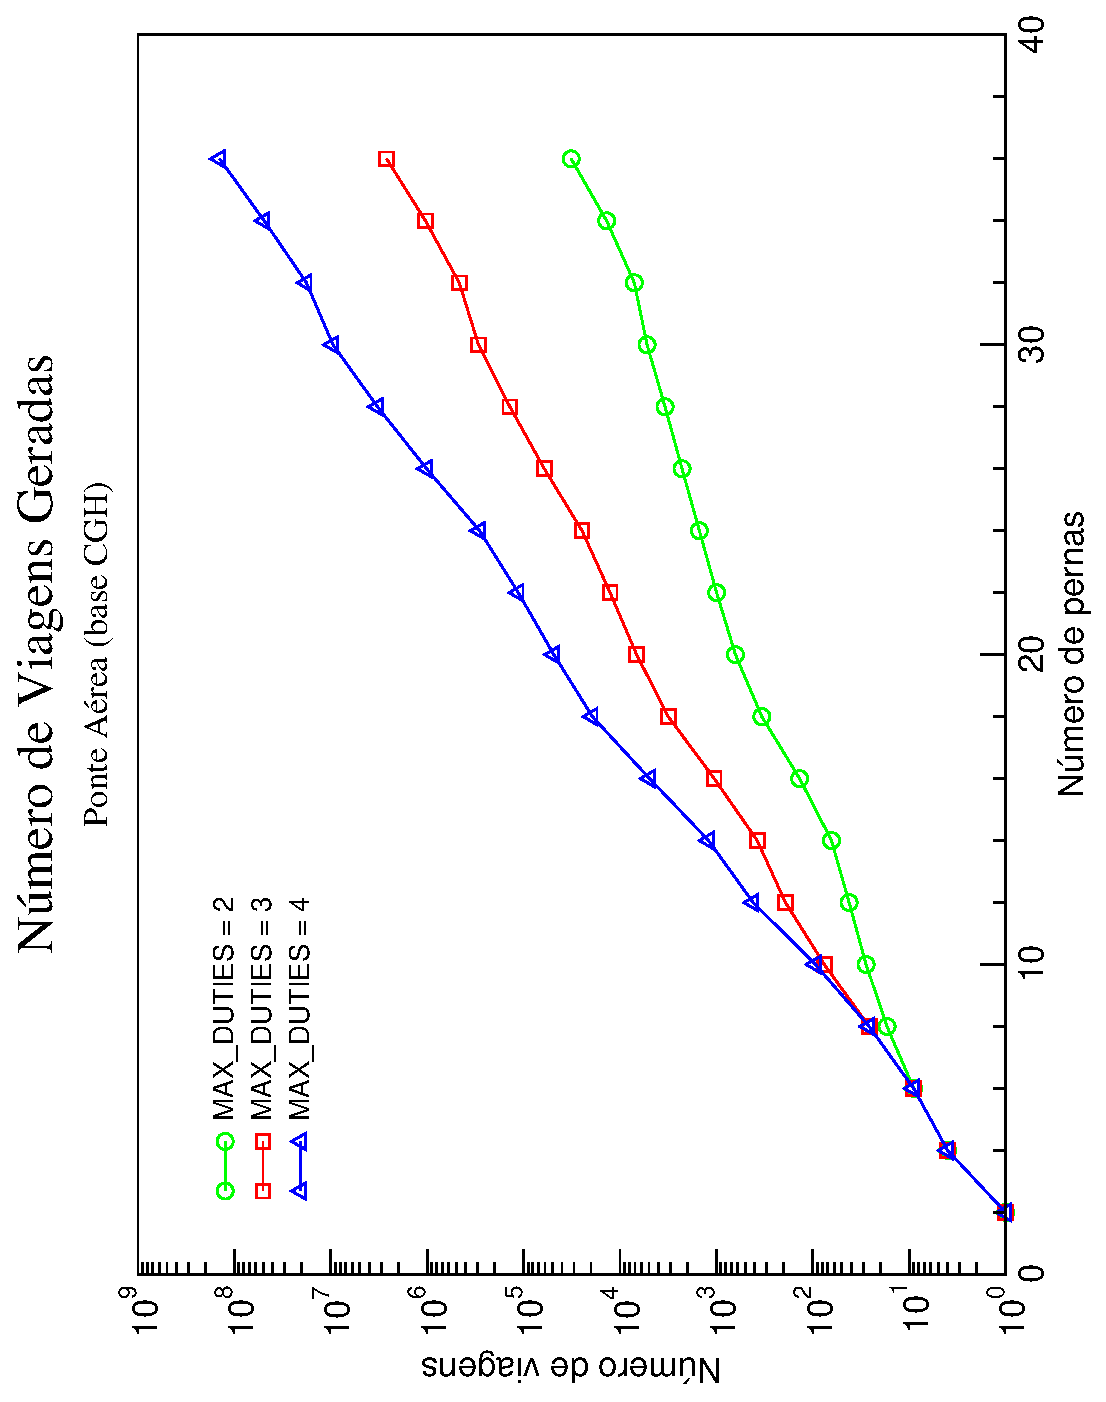
\includegraphics[scale=0.45,angle=-90]{fig/number_of_pairings.eps}
		\caption{Número de viagens geradas em função do número de pernas utilizadas na construção da
		rede de voos. Note a escala logarítmica do eixo vertical.}
		\label{fig:pairings}
	\end{center}
\end{figure}

O consumo de tempo gasto pelo algoritmo de busca em profundidade também foi medido em função do 
número de pernas. Os resultados são apresentados na Figura~\ref{fig:generation}. O comportamento das
curvas indicam também um crescimento exponencial do tempo gasto pelo algoritmo, ainda que ele seja
executado de forma rápida (para \verb|MAX_DUTIES| = 4, encontrou-se um tempos da ordem de $10^4$~ms 
para 36 pernas).

\begin{figure}[htb]
	\begin{center}
		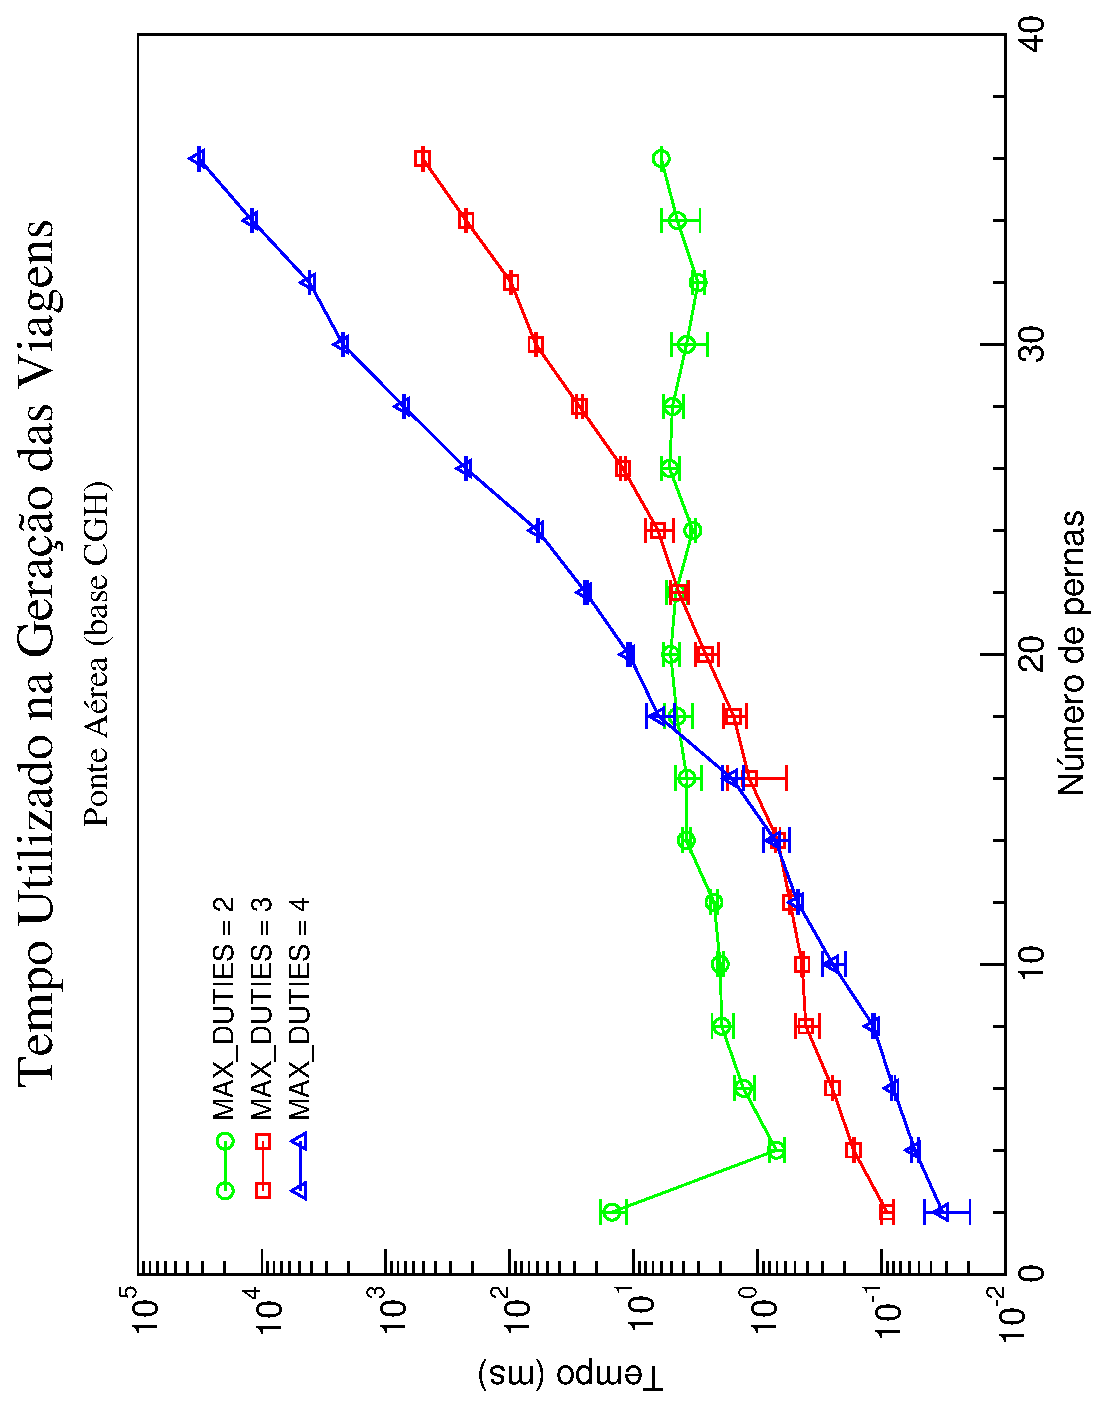
\includegraphics[scale=0.45,angle=-90]{fig/generation_time.eps}
		\caption{Tempo gasto na geração das viagens em função do número de pernas utilizadas na 
		construção da rede de voos. São apresentados valor médio $\pm$ desvio-padrão, considerando 5 
		medidas para cada ponto. Note a escala logarítmica do eixo vertical.}
		\label{fig:generation}
	\end{center}
\end{figure}

%%%%%%%%%%%%%%%%%%%%%%%%%%%%%%%%%%%%%%%%%%%%%%%%%%%%%%%%%%%%%%%%%%%%%%%%%%%%%%%%%%%%%%%%%%%%%%%%%%%%

\section{Otimização}
\label{sec:otimizacao}

As viagens geradas são levadas ao processo de otimização resolvendo-se um modelo de programação 
linear inteira. Esse modelo busca minimizar o custo das viagens de forma que cada perna do conjunto
de voos seja coberta exatamente uma vez. 

O custo de uma viagem foi calculado como sendo o tempo ``ocioso'' no qual o tripulante está 
trabalhando mas não está voando, ou seja, pela diferença entre o tempo total de uma viagem, menos o 
tempo total de voo efetuado, descontando ainda os tempos mínimos regulamentares de conexão entre 
pernas e de descanso entre jornadas. Esse custo avalia de forma estimada a produtividade de uma 
viagem.

Foi utilizado o otimizador GLPK (GNU Linear Programming Kit), versão~4.47, com a adoção de um 
esquema de relaxação para resolver o PL associado (simplex primal), seguido de uma estratégia 
branch-and-bound para encontrar soluções inteiras.

O tempo gasto pelo otimizador para resolver o modelo proposto é apresentado no gráfico da 
Figura~\ref{fig:solution}, variando-se o número de pernas em cada instância considerada. 
Mais uma vez, observa-se um crescimento exponencial muito forte (note a escala logarítmica do eixo 
vertical), mostrando que a resolução do modelo se torna impraticável para instâncias com um número 
de pernas da ordem de~40.

\begin{figure}[htb]
	\begin{center}
		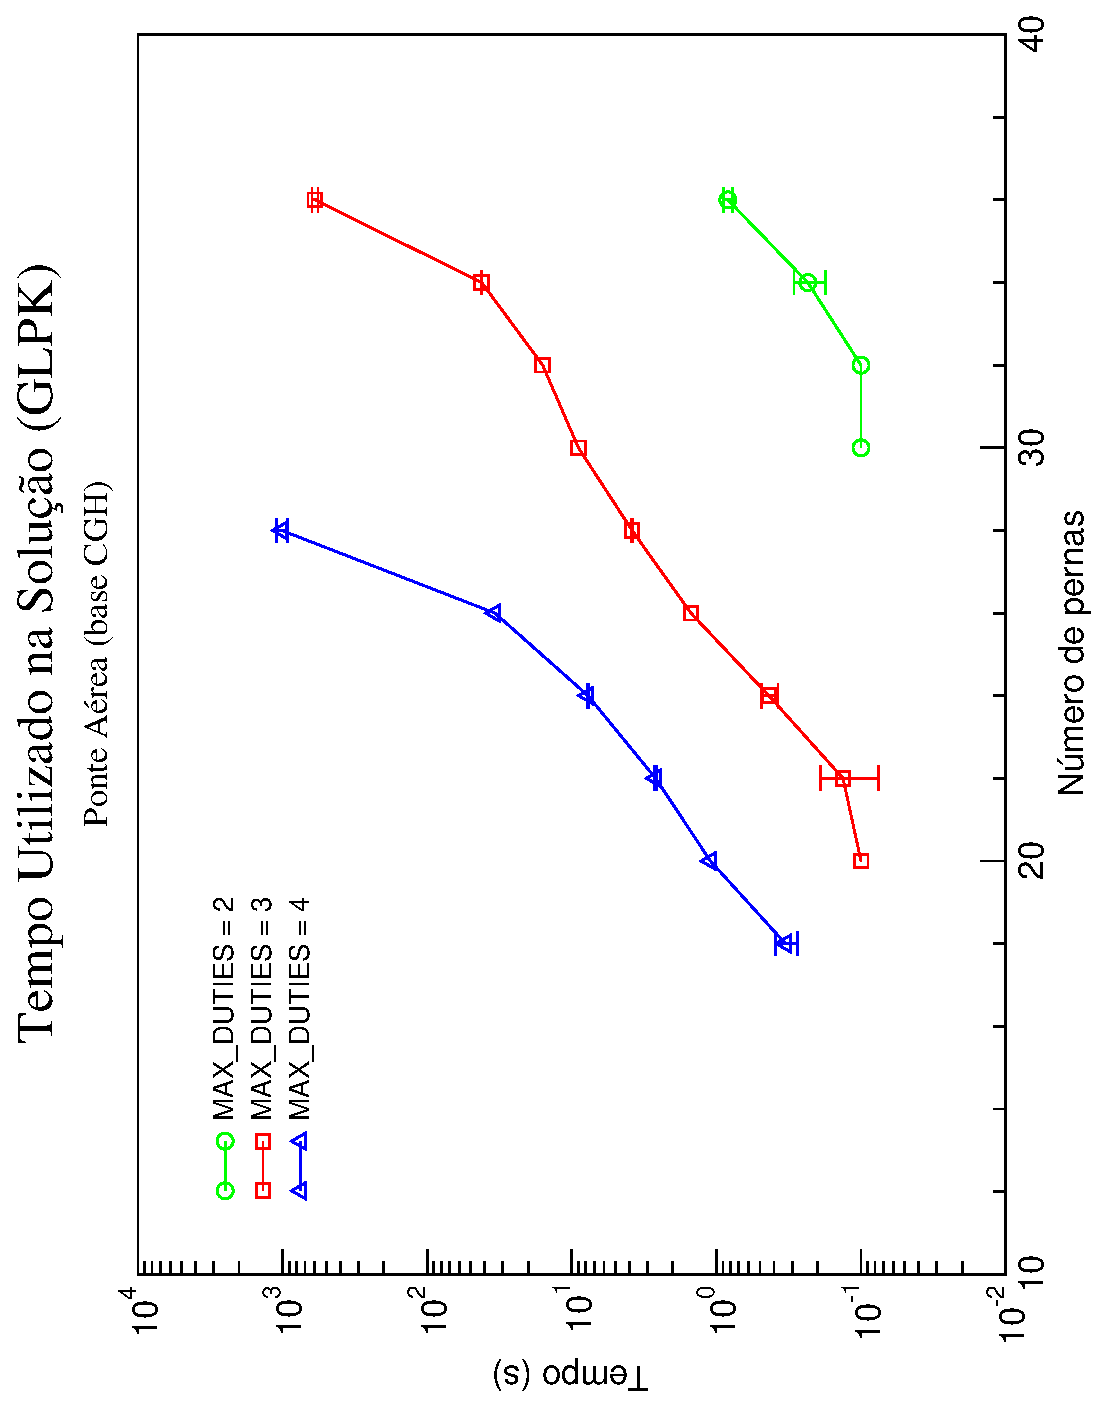
\includegraphics[scale=0.45,angle=-90]{fig/glpk_solution_time.eps}
		\caption{Tempo utilizado pelo otimizador GLPK na obtenção de uma solução inteira, em função do 
		número de pernas utilizadas na construção da rede de voos. São apresentados valor médio $\pm$ 
		desvio-padrão, considerando 3 medidas para cada ponto. Valores medidos com tempo de execução 
		de 0,0~s não são apresentados (número pequeno de pernas). O último ponto (36 pernas) da curva 
		azul não pode ser estimado, mesmo após 5 horas de processamento.}
		\label{fig:solution}
	\end{center}
\end{figure}

%%%%%%%%%%%%%%%%%%%%%%%%%%%%%%%%%%%%%%%%%%%%%%%%%%%%%%%%%%%%%%%%%%%%%%%%%%%%%%%%%%%%%%%%%%%%%%%%%%%%

\section{Conclusões}
\label{sec:conclusoes}

Dos resultados apresentados, concluímos que o procedimento de geração de viagens leva a um número 
gigantesco de variáveis, mesmo para um pequeno número de pernas. Isso porque a natureza combinatória 
do problema leva o algoritmo de busca a explorar diversas possibilidades, principalmente em uma rede 
como a da ponte aérea, onde existem diversas possibilidades de conexão toda vez que se chega em uma
das localidades. Além disso, essas possibilidades se multiplicam quando consideramos um maior número
de jornadas permitidas (\verb|MAX_DUTIES|). Apesar disso, a geração de viagens ainda se fez em tempo 
aceitável, podendo ser aplicada para redes maiores. 

Entretanto, quando esse número enorme de variáveis é levado ao otimizador, o tempo de processamento 
se torna impraticável. Ainda assim, ficamos surpresos com a capacidade do otimizador resolver 
instâncias com um número de variáveis da ordem de $10^6$ em tempo aceitável. Na verdade, após uma
análise mais profunda, percebeu-se muita redundância nas colunas geradas (mesmas colunas com custos 
diferentes), as quais eram prontamente eliminadas durante a fase de pre-processamento do otimizador.
Além disso, apesar do número de colunas ser grande, o número de linhas ainda é bem pequeno, o que
facilita bastante o trabalho do otimizador.

Dessa forma, procedimentos heurísticos devem ser adotados desde a fase de geração (conforme 
discutido na literatura) com o objetivo de se reduzir o número de colunas redundantes, bem como das
colunas muito custosas. Duas alternativas a serem exploradas são:

\begin{itemize}
	\item Limitação do número de troca de aeronaves por jornada: forçamos com isso a tripulação
	acompanhar, na medida do possível, o trilho percorrido pela aeronave, reduzindo a possibilidade de
	conexões em cada localidade. Naturalmente os tempos de conexão serão reduzidos, tornando as 
	viagens geradas mais baratas e diminuindo o número total de variáveis geradas. Além disso, esse 
	procedimento torna a solução mais robusta, uma vez que o atraso de uma aeronave não acarretará 
	atraso na saída de outro voo que dependa daquela aeronave na troca. 
	\item Cutoff no custo das viagens geradas: um caminho legal encontrado que represente um custo 
	muito alto com relação ao total de horas voadas será automaticamente descartada, se passar de um 
	determinado limiar. Viagens caras apresentam poucas chances de serem selecionadas pelo otimizador, 
	de forma que podemos eliminá-las {\it a priori} do processo de otimização.
\end{itemize}

Com isso, conseguiremos instâncias com um número maior de linhas e menor de colunas que podem ser
utilizadas para testar melhor a performance do otimizador, tornando a análise mais realista.
Pretende-se ainda realizar os mesmos testes utilizando um otimizador mais robusto como o CPLEX da 
IBM.

%%%%%%%%%%%%%%%%%%%%%%%%%%%%%%%%%%%%%%%%%%%%%%%%%%%%%%%%%%%%%%%%%%%%%%%%%%%%%%%%%%%%%%%%%%%%%%%%%%%%

\end{document}